\documentclass[11pt,a4paper]{article}
\usepackage{fullpage}
\usepackage{tabu}
\usepackage[utf8]{inputenc}
\usepackage{tikz,xstring}
\usepackage{pgf}
\usetikzlibrary{arrows,automata}
\usetikzlibrary{positioning}
\title{Beastly Heis v1.5}
\author{Kolbjørn Austreng, Andreas Våge}
\tikzset{
    state/.style={
           rectangle,
           rounded corners,
           draw=black, very thick,
           minimum height=2em,
           inner sep=2pt,
           text centered,
           },
}

\begin{document}
\maketitle
\section*{Diagrams}
\begin{figure}[h]
\centering
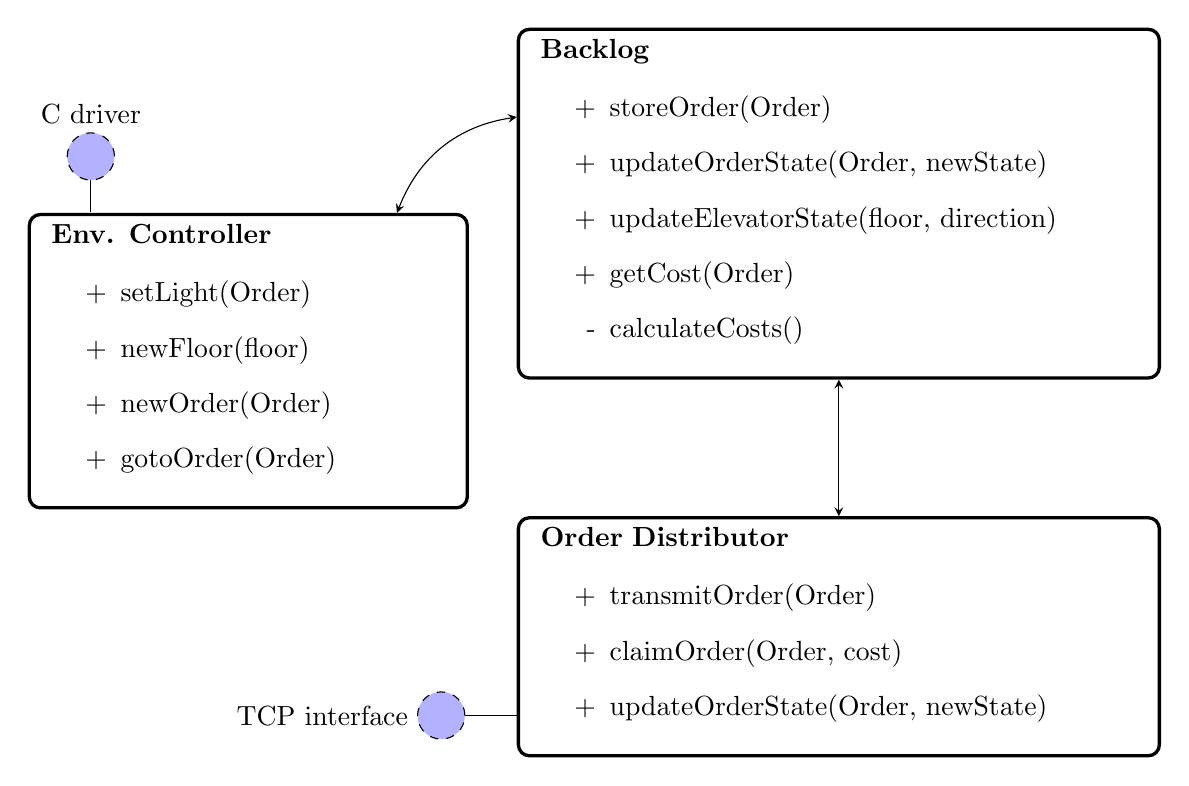
\begin{tikzpicture}[->,>=stealth]

 % Position of Env Controller 
 % Use previously defined 'state' as layout (see above)
 % use tabular for content to get columns/rows
 % parbox to limit width of the listing
 \node[state] (Env Controller)
 {\begin{tabular}{l}
  \textbf{Env. Controller}\\
  \parbox{5cm}{\begin{itemize}
   \item[+] setLight(Order)
	\item[+] newFloor(floor)
	\item[+] newOrder(Order)
	\item[+] gotoOrder(Order)
  \end{itemize}
  }
 \end{tabular}};

 \node[state,       % layout (defined above)
  text width=8cm,   % max text width
  yshift=2cm,       % move 2cm in y
  right of=Env Controller,   
  node distance=7.5cm,  
  anchor=center] (Backlog)  % posistion relative to the center of the 'box'
  {\begin{tabular}{l}
  \textbf{Backlog}\\
  \parbox{8cm}{\begin{itemize}
   \item[+] storeOrder(Order)
   \item[+] updateOrderState(Order, newState)
   \item[+] updateElevatorState(floor, direction)
   \item[+] getCost(Order)
   \item[-] calculateCosts()

  \end{itemize}
  }
 \end{tabular}};
 
 % STATE Communication
 \node[state,
  below of=Backlog,
  yshift=-4.5cm,
  anchor=center,
  text width=8cm] (Communication) 
 {\begin{tabular}{l}
  \textbf{Order Distributor}\\
  \parbox{8cm}{\begin{itemize}
   \item[+] transmitOrder(Order)
   \item[+] claimOrder(Order, cost)
   \item[+] updateOrderState(Order, newState)

  \end{itemize}
  }
 \end{tabular}};

 
 % draw the paths and and print some Text below/above the graph
 \path[<->] (Env Controller)  edge[bend left=30]   (Backlog)
 %(Env Controller)        edge[bend right=20]  (Communication)
 %(Communication)     edge[loop below]    node[anchor=north,below]{$SC_n\neq 0$} (Communication)
 (Communication)     edge                 (Backlog);

% Tacked on orbital data
\begin{scope}[-]
\begin{scope}[xshift=0.8cm,yshift=-0.4cm]
\path[draw] (-2.8,2.3) -- (-2.8,3);
\path[draw,dashed, fill = blue!30] (-2.8, 3) circle (0.3) node[above = 0.3cm] {C driver};
\end{scope}
\path[draw] (3.45,-4.5) -- (2.45,-4.5);
\path[draw,dashed, fill = blue!30] (2.45,-4.5) circle (0.3) node[left = 0.3cm] {TCP interface};
\end{scope}
\end{tikzpicture}
\caption{System module diagram.}
\end{figure}
\begin{figure}[h]
  \centering
  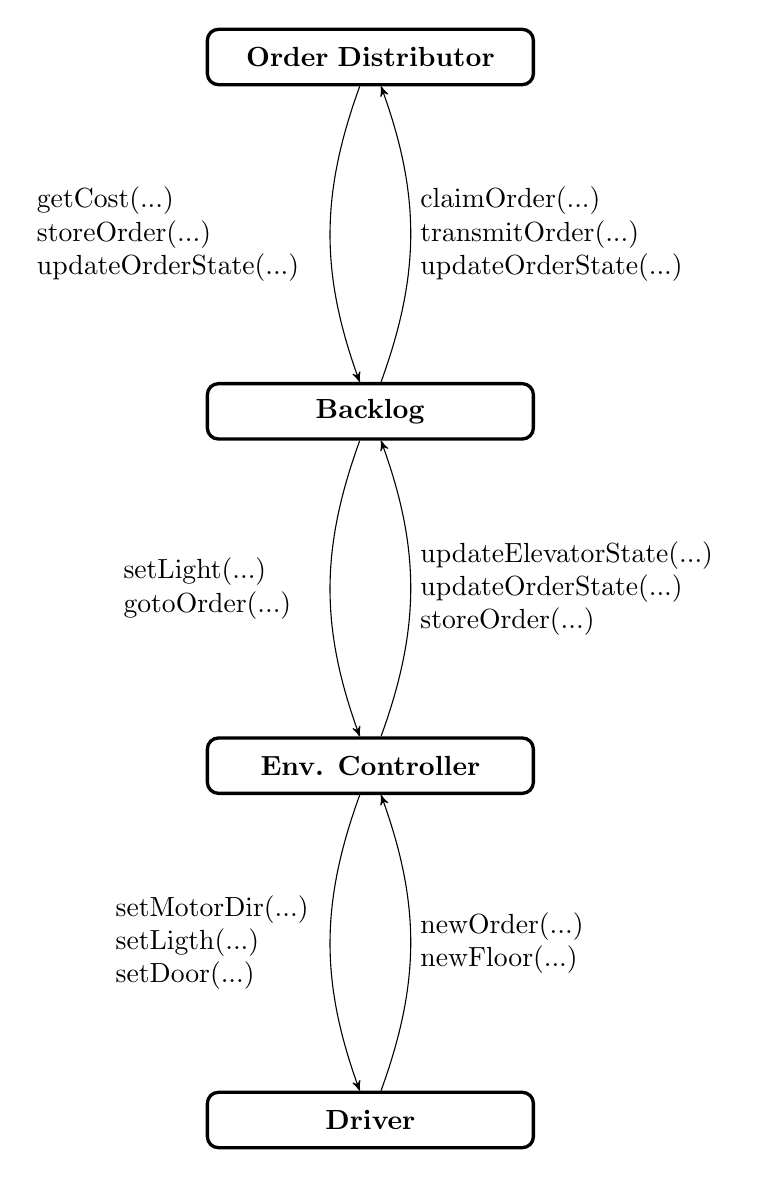
\begin{tikzpicture}[->,>=stealth']

 % Position of Env Controller 
 % Use previously defined 'state' as layout (see above)
 % use tabular for content to get columns/rows
 % parbox to limit width of the listing
 \node[state,text width=4cm] (Env Controller) 
 {\textbf{Env. Controller}};

 \node[state,       % layout (defined above)
  text width=4cm,   % max text width      
  above of=Env Controller,   
  node distance=4.5cm,  
  anchor=center] (Backlog)  % posistion relative to the center of the 'box'
  {\textbf{Backlog}};
 
 % STATE Communication
 \node[state,
  above of=Backlog,
  node distance=4.5cm,
  anchor=center,
  text width=4cm] (Communication) 
 {\textbf{Order Distributor}};

 \node[state,
  below of=Env Controller,
  node distance=4.5cm,
  anchor=center,
  text width=4cm] (Driver) 
 {\textbf{Driver}};

 
 % draw the paths and and print some Text below/above the graph
 \draw[<-] (Env Controller) edge[bend left=20] node[pos=0.5,left]{\parbox{2.5cm}{setLight(...)\\gotoOrder(...)}}(Backlog);
 \draw[->](Env Controller) edge[bend right=20] node[pos=0.5,right]{\parbox{4cm}{updateElevatorState(...)\\updateOrderState(...)\\storeOrder(...)}} (Backlog);

 \draw[->](Communication) edge[bend right=20] node[pos=0.5,left]{\parbox{3.6cm}{getCost(...)\\storeOrder(...)\\updateOrderState(...)}} (Backlog);
 \draw[<-](Communication) edge[bend left=20] node[pos=0.5,right]{\parbox{3.6cm}{claimOrder(...)\\transmitOrder(...)\\updateOrderState(...)}} (Backlog);

 \draw[->](Env Controller) edge[bend right=20] node[pos=0.5,left]{\parbox{2.6cm}{setMotorDir(...)\\setLigth(...)\\setDoor(...)}} (Driver);
 \draw[<-](Env Controller) edge[bend left=20] node[pos=0.5,right]{\parbox{3cm}{newOrder(...)\\newFloor(...)}} (Driver);

\end{tikzpicture}
\caption{Function call between modules}
\end{figure}


\begin{figure}[h]
  \centering
  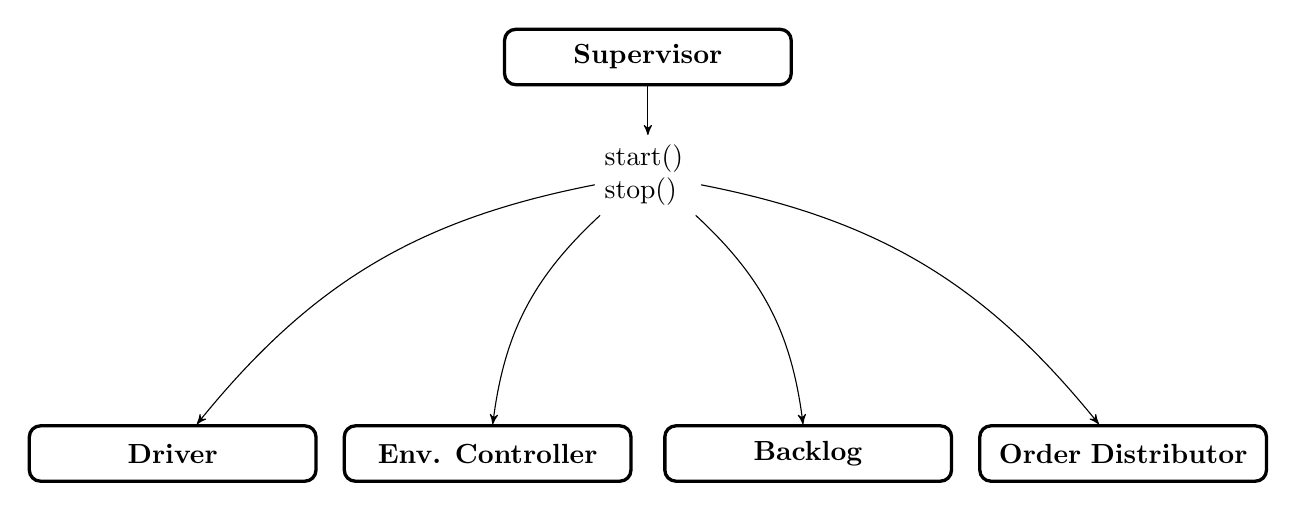
\begin{tikzpicture}[->,>=stealth']
 \node[] (Supervisor) 
 {\parbox{1.1cm}{start()\\stop()}};

 \node[state,
  above of=Supervisor,
  node distance=1.5cm,  
  anchor=center,
  text width=3.5cm] (SUPERVISOR) 
 {\textbf{Supervisor}};

 \node[state,
  below left of=Supervisor,
  node distance=5cm,
  xshift=1.5cm,   
  anchor=center,
  text width=3.5cm] (Env Controller) 
 {\textbf{Env. Controller}};

 \node[state,       % layout (defined above)
  text width=3.5cm,   % max text width      
  below right of=Supervisor,
  xshift=-1.5cm,   
  node distance=5cm,  
  anchor=center] (Backlog)  % posistion relative to the center of the 'box'
  {\textbf{Backlog}};
 
 % STATE Communication
 \node[state,
  right of=Backlog,
  node distance=4cm,
  anchor=center,
  text width=3.5cm] (Communication) 
 {\textbf{Order Distributor}};

 \node[state,
  left of=Env Controller,
  node distance=4cm,
  anchor=center,
  text width=3.5cm] (Driver) 
 {\textbf{Driver}};

 
 % draw the paths and and print some Text below/above the graph
 
 \draw[->](Supervisor) edge[bend right=20] node[pos=0.5,left]{} (Driver);
 \draw[->](Supervisor) edge[bend right=20] node[pos=0.5,left]{} (Env Controller);
 \draw[->](Supervisor) edge[bend left=20] node[pos=0.5,left]{} (Backlog);
 \draw[->](Supervisor) edge[bend left=20] node[pos=0.5,left]{} (Communication);
 \draw[->](SUPERVISOR) edge node[pos=0.5,left]{} (Supervisor);

\end{tikzpicture}
\caption{Supervisor}
\end{figure}



\begin{figure}[h]
\centering
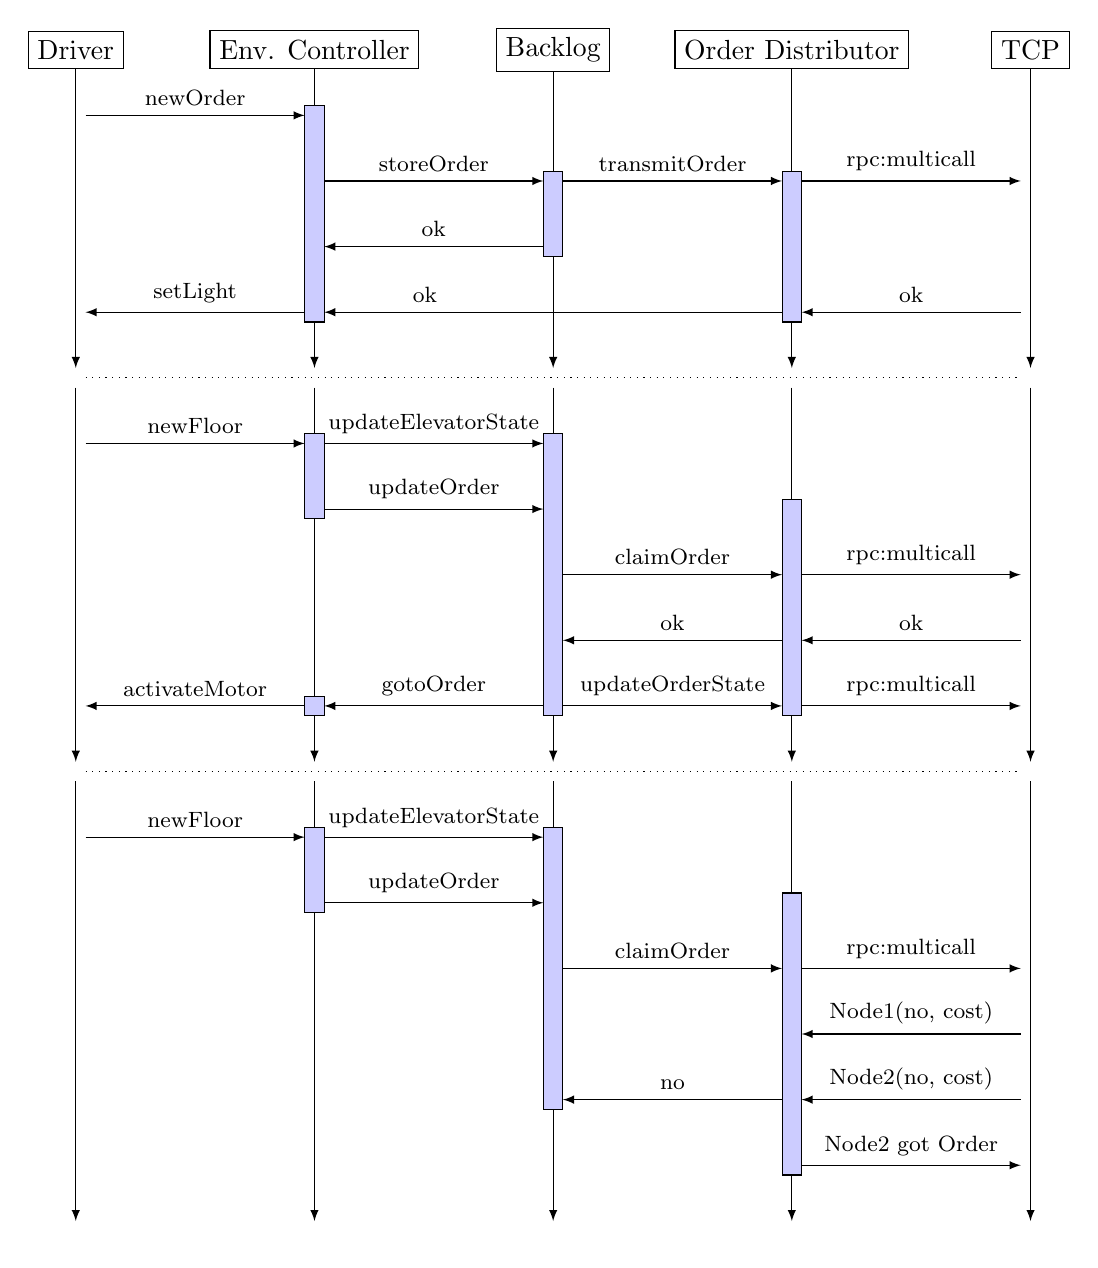
\begin{tikzpicture}

  \def\numberOfRows{18}
  % Agents
  \def\AgentList{Driver,Env. Controller,Backlog,Order Distributor, TCP}

  %determining the space betwen each point in the matrix
  \def\spaceRows{\textwidth/\numberOfColums} 
  \def\spaceColums{15/\numberOfRows}

  %Calculating stuff
  \StrCount{\AgentList}{,}[\arrlength]
  \def\numberOfColums{\arrlength}
  %Matrix
    \foreach \x in {0,...,\numberOfColums}
      \foreach \y in {0,...,\numberOfRows} 
         {\node(\x\y) at (\spaceRows*\x,-\spaceColums*\y) {};} %Label \x:\y when working, empty when done


  % Vertical lifelines
  \foreach \x in {0,...,\numberOfColums}
      {\draw [-latex] (\x0) -- (\x5);
      \draw [-latex] (\x5) -- (\x11);
      \draw [-latex] (\x11) -- (\x\numberOfRows);}

  %Agents labels
  \foreach \c [count=\x from 0] in \AgentList
      \fill (\x0) node[draw,fill=white] {\c};
      

  % Blocks 
  \filldraw[fill=blue!20]
     (11.north west) rectangle (14.south east)
     (22.north west) rectangle (23.south east)
     (32.north west) rectangle (34.south east);

  \filldraw[fill=blue!20]
     (16.north west) rectangle (17.south east)
     (26.north west) rectangle (210.south east)
     (37.north west) rectangle (310.south east)
     (110.north west) rectangle (110.south east);

  \filldraw[fill=blue!20]
     (112.north west) rectangle (113.south east)
     (212.north west) rectangle (216.south east)
     (313.north west) rectangle (317.south east);


  % Horizontal flows
  %Store Order
  \draw [-latex] (01) -- node[pos=0.5,font=\footnotesize, above] {newOrder} (11);
  \draw [-latex] (12) -- node[pos=0.5,font=\footnotesize, above] {storeOrder} (22);
  \draw [-latex] (22) -- node[pos=0.5,font=\footnotesize, above] {transmitOrder} (32);
  \draw [-latex] (32) -- node[pos=0.5,font=\footnotesize, above] {rpc:multicall} (42);
  \draw [-latex] (44) -- node[pos=0.5,font=\footnotesize, above] {ok} (34);
  \draw [-latex] (23) -- node[pos=0.5,font=\footnotesize, above] {ok} (13);
  \draw [-latex] (34) -- node[pos=0.78,font=\footnotesize, above] {ok} (14);
  \draw [-latex] (14) -- node[pos=0.5,font=\footnotesize, above] {setLight} (04);

  \draw [dotted]  (05) -- (45);
  %
  \draw [-latex] (06) -- node[pos=0.5,font=\footnotesize, above] {newFloor} (16);
  \draw [-latex] (16) -- node[pos=0.5,font=\footnotesize, above] {updateElevatorState} (26);
  \draw [-latex] (17) -- node[pos=0.5,font=\footnotesize, above] {updateOrder} (27);
  \draw [-latex] (28) -- node[pos=0.5,font=\footnotesize, above] {claimOrder} (38);
  \draw [-latex] (38) -- node[pos=0.5,font=\footnotesize, above] {rpc:multicall} (48);
  \draw [-latex] (49) -- node[pos=0.5,font=\footnotesize, above] {ok} (39);
  \draw [-latex] (39) -- node[pos=0.5,font=\footnotesize, above] {ok} (29);
  \draw [-latex] (210) -- node[pos=0.5,font=\footnotesize, above] {updateOrderState} (310);
  \draw [-latex] (310) -- node[pos=0.5,font=\footnotesize, above] {rpc:multicall} (410);
  \draw [-latex] (210) -- node[pos=0.5,font=\footnotesize, above] {gotoOrder} (110);
  \draw [-latex] (110) -- node[pos=0.5,font=\footnotesize, above] {activateMotor} (010);

  \draw [dotted]  (011) -- (411);

  \draw [-latex] (012) -- node[pos=0.5,font=\footnotesize, above] {newFloor} (112);
  \draw [-latex] (112) -- node[pos=0.5,font=\footnotesize, above] {updateElevatorState} (212);
  \draw [-latex] (113) -- node[pos=0.5,font=\footnotesize, above] {updateOrder} (213);
  \draw [-latex] (214) -- node[pos=0.5,font=\footnotesize, above] {claimOrder} (314);
  \draw [-latex] (314) -- node[pos=0.5,font=\footnotesize, above] {rpc:multicall} (414);
  \draw [-latex] (415) -- node[pos=0.5,font=\footnotesize, above] {Node1(no, cost)} (315);
  \draw [-latex] (416) -- node[pos=0.5,font=\footnotesize, above] {Node2(no, cost)} (316);
  \draw [-latex] (316) -- node[pos=0.5,font=\footnotesize, above] {no} (216);
  \draw [-latex] (317) -- node[pos=0.5,font=\footnotesize, above] {Node2 got Order} (417);
\end{tikzpicture}
\caption{Sequence diagram between modules}
\end{figure}
\clearpage
\begin{figure}[h]
  \centering  
  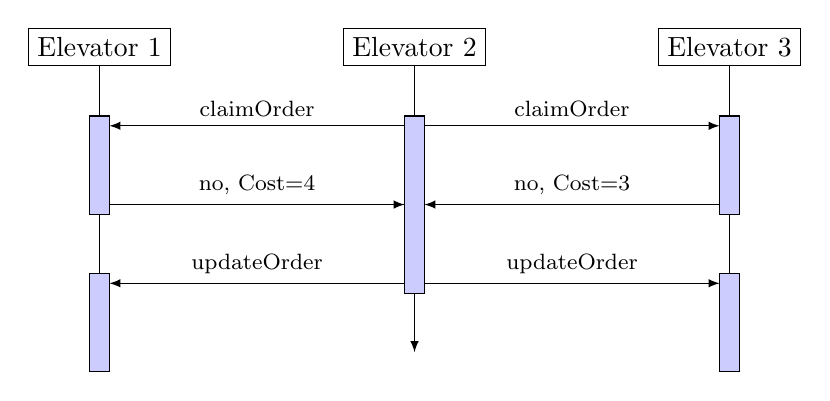
\begin{tikzpicture}

  \def\numberOfRows{4}
  % Agents
  \def\AgentList{Elevator 1, Elevator 2, Elevator 3}

  %determining the space betwen each point in the matrix
  \def\spaceRows{8/\numberOfColums} 
  \def\spaceColums{4/\numberOfRows}

  %Calculating stuff
  \StrCount{\AgentList}{,}[\arrlength]
  \def\numberOfColums{\arrlength}
  %Matrix
    \foreach \x in {0,...,\numberOfColums}
      \foreach \y in {0,...,\numberOfRows} 
         {\node(\x\y) at (\spaceRows*\x,-\spaceColums*\y) {};} %Label \x:\y when working, empty when done


  % Vertical lifelines
  \foreach \x in {0,...,\numberOfColums}
      {\draw [-latex] (\x0) -- (\x\numberOfRows);}

  %Agents labels
  \foreach \c [count=\x from 0] in \AgentList
      \fill (\x0) node[draw,fill=white] {\c};
      

 
  % Horizontal flows
  \draw [-latex] (11) -- node[pos=0.5,font=\footnotesize, above] {claimOrder} (21);
  \draw [-latex] (11) -- node[pos=0.5,font=\footnotesize, above] {claimOrder} (01);
  \draw [-latex] (02) -- node[pos=0.5,font=\footnotesize, above] {no, Cost=4} (12);
  \draw [-latex] (22) -- node[pos=0.5,font=\footnotesize, above] {no, Cost=3} (12);
  \draw [-latex] (13) -- node[pos=0.5,font=\footnotesize, above] {updateOrder} (23);
  \draw [-latex] (13) -- node[pos=0.5,font=\footnotesize, above] {updateOrder} (03);
  
   % Blocks 
  \filldraw[fill=blue!20] 
  (11.north west) rectangle (13.south east)
  (21.north west) rectangle (22.south east)
  (01.north west) rectangle (02.south east)
  (23.north west) rectangle (24.south east)
  (03.north west) rectangle (04.south east);
\end{tikzpicture}
\caption{Sequence diagram between three elevators}
\end{figure}

\begin{figure}[h]
\centering
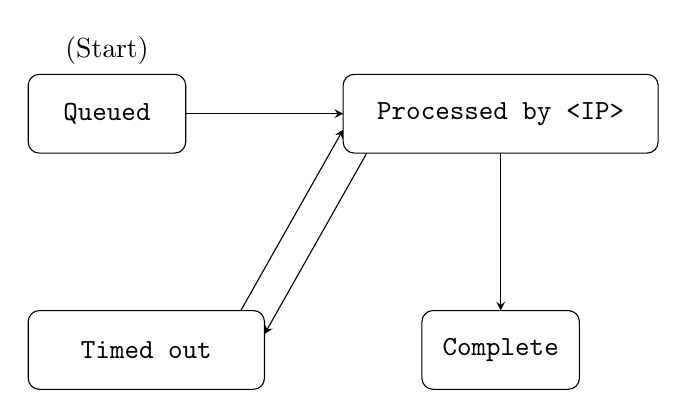
\begin{tikzpicture}[>=stealth]
\path[draw, rounded corners, fill = white] (0,4) rectangle (2,5) node[midway] {\verb!Queued!};
\path[draw, rounded corners, fill = white] (4,4) rectangle ++(4,1) node[midway] {\verb!Processed by <IP>!};
\path[draw, rounded corners, fill = white] (0,1) rectangle ++(3,1) node[midway] {\verb!Timed out!};
\path[draw, rounded corners, fill = white] (5,1) rectangle ++(2,1) node[midway] {\verb!Complete!};
\path[draw,->] (2,4.5) -- ++(2,0);
\path[draw,->] (6, 4) -- ++(0,-2);
\path[draw,->] (4.3,4) -- (3,1.7);
\path[draw,->] (2.7,2) -- (4,4.3);
\path (1,5) node[above] {(Start)};
\end{tikzpicture}
\caption{Order life stages.}
\end{figure}

\section*{Order object}
\begin{tabu}{|X|X|}
\hline
\textbf{Order} & Comment\\ \hline
+ type & Internal / External\\
+ floor & Destination floor\\
+ timestamp & Set by computer that first received order\\
+ origin IP & Set by computer that first received order\\
+ state & Queued, In progress, Timed out, Complete\\ \hline
\end{tabu}
\section*{Environment Controller}
\subsubsection*{+ setLight(Order)}
Sets the light corresponding to the floor of an Order object.
\subsubsection*{+ newFloor(int floor)}
Call from C driver to communicate to \textit{Environment Controller} that a new floor has been reached.
\subsubsection*{+ newOrder(Order)}
Call from C driver to communicate to \textit{Environment Controller} that a new order has been created.
\subsubsection*{+ gotoOrder(Order)}
Sends the elevator to the floor of a specific order.
\section*{Backlog}
\subsubsection*{+ storeOrder(Order) ok}
Saves an order from either \textit{Environment Controller} or \textit{Order Distributor} to the backlog. Returns acknowledgement.
\subsubsection*{+ updateOrderState(Order, newState) ok}
Changes the state of a specific order. Returns acknowledgement.
\subsubsection*{+ updateElevatorState(int floor, enum direction)}
Communicates the position and direction of the elevator to the \textit{Backlog}.
\subsubsection*{+ getCost(Order) cost}
Returns the cost of taking a specific order for this elevator.
\subsubsection*{- calculateCosts()}
Calculates the costs of all the orders in the backlog for this elevator.
\section*{Order Distributor}
\subsubsection*{+ transmitOrder(Order) ok}
Transmits an Order object to all the other nodes in the network. Acknowledges if at least one other elevator received the order transmit, or there are no other elevators in the network.
\subsubsection*{+ claimOrder(Order, cost) ok}
Attempts to claim an order in the \textit{Backlog}. Transmits own cost of taking on this order. Acknowledges if no other elevators have a lower cost on the specified order.
\subsubsection*{+ updateOrderState(Order, newState) ok}
Broadcasts an order state update to ensure that the backlogs are identical.
\clearpage
\section*{Fault handling}
\subsubsection*{Software crash}
\begin{itemize}
\item Backlog is saved to a local file.
\item All orders are distributed to all other nodes.
\item Upon restart, open saved backlog, merge with network backlog.
\item All claimed orders will time out; be claimed by other nodes.
\end{itemize}
\subsubsection*{Software hangs}
\begin{itemize}
\item Time out on claimed orders.
\item Supervisor restarts process.
\end{itemize}
\subsubsection*{Network cable disconnect, then reconnect}
\begin{itemize}
\item Claimed orders time out when TCP marks it as dead.
\item Syncs backlog from network on reconnect.
\end{itemize}
\subsubsection*{Troll user}
\begin{itemize}
\item Cost function prioritizes continuing in current direction, and older orders. An elevator will never not serve an order, given enough time.
\end{itemize}
\subsubsection*{Elevator never arrives}
\begin{itemize}
\item Order times out, different elevator takes over.
\end{itemize}
\subsubsection*{Cosmic rays}
\begin{itemize}
\item TCP for detecting junked up messages.
\item New "phantom" orders may be created, no big deal.
\item No orders can be wiped from the system without being explicitly marked as complete.
\item Supervisor restarts uncooperative processes.
\end{itemize}
\subsubsection*{Power out on all elevators}
\begin{itemize}
\item Backlog saved to local file, will carry on where they left of on power up.
\end{itemize}
\subsubsection*{Heat Death of the Universe}
\begin{itemize}
\item This is acceptable.
\end{itemize}
\end{document}